% Software Design 24
% 2.1 Application Architecture . . . . . . . . . . . . . . . . . . . . . . . . . . 24
% 2.1.1 Architectural Design . . . . . . . . . . . . . . . . . . . . . . . . 24
% 2.1.2 Decomposition Description . . . . . . . . . . . . . . . . . . . . . 25
% 2.2 Data Design . . . . . . . . . . . . . . . . . . . . . . . . . . . . . . . . . 25
% 2.2.1 Data Description . . . . . . . . . . . . . . . . . . . . . . . . . . 25

% 2.2.2 Data Dictionary . . . . . . . . . . . . . . . . . . . . . . . . . . . 30
\section{Software Design}
\subsubsection{Application Architecture }
\begin{figure}[H]
    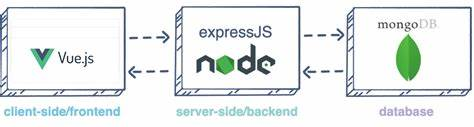
\includegraphics[width=\linewidth]{ARCHTURE.jpg }
    \caption{ Application Architecture}
    \label{fig:Application-Architecture}
\end{figure}

\section[]{Decomposition Description}

\begin{tikzpicture}[
        block/.style={
                rectangle,
                draw,
                text width=6em,
                text centered,
                minimum height=4em
            },
        line/.style={
                draw,
                -latex'
            }
    ]

    \node [block] (app) {E-commerce Application};

    \node [block, below=2cm of app] (user) {User Use Cases};
    \node [block, below=of user] (auth) {User Authentication};
    \node [block, right=of auth] (reg) {Register};
    \node [block, right=of reg] (login) {Login};
    \node [block, below=of auth] (browse) {Product Browsing};
    \node [block, right=of browse] (view) {View Products};
    \node [block, right=of view] (search) {Search Products};
    \node [block, below=of browse] (wishlist) {Wishlist};
    \node [block, right=of wishlist] (addWish) {Add to Wishlist};
    \node [block, right=of addWish] (viewWish) {View Wishlist};
    \node [block, below=of wishlist] (basket) {Basket};
    \node [block, right=of basket] (addBasket) {Add to Basket};
    \node [block, right=of addBasket] (viewBasket) {View Basket};
    \node [block, below=of basket] (order) {Order};
    \node [block, right=of order] (track) {Track Order Status};
    \node [block, right=of track] (viewOrder) {View Order Information};

    \node [block, below=2cm of user] (admin) {Admin Use Cases};
    \node [block, below=of admin] (prod) {Product Management};
    \node [block, right=of prod] (addProd) {Add Product};
    \node [block, right=of addProd] (editProd) {Edit Product};
    \node [block, below=of prod] (ord) {Order Management};
    \node [block, right=of ord] (viewOrd) {View Order};
    \node [block, right=of viewOrd] (updateOrd) {Update Order Status};

    \path [line] (app) -- (user);
    \path [line] (user) -- (auth);
    \path [line] (auth) -- (reg);
    \path [line] (reg) -- (login);
    \path [line] (user) -- (browse);
    \path [line] (browse) -- (view);
    \path [line] (view) -- (search);
    \path [line] (user) -- (wishlist);
    \path [line] (wishlist) -- (addWish);
    \path [line] (addWish) -- (viewWish);
    \path [line] (user) -- (basket);
    \path [line] (basket) -- (addBasket);
    \path [line] (addBasket) -- (viewBasket);
    \path [line] (user) -- (order);
    \path [line] (order) -- (track);
    \path [line] (track) -- (viewOrder);

    \path [line] (app) -- (admin);
    \path [line] (admin) -- (prod);
    \path [line] (prod) -- (addProd);
    \path [line] (addProd) -- (editProd);
    \path [line] (admin) -- (ord);
    \path [line] (ord) -- (viewOrd);
    \path [line] (viewOrd) -- (updateOrd);

\end{tikzpicture}

This diagram breaks down the e-commerce application into its main components:
User Authentication, Product Browsing, Wishlist, Basket, Order, Product Management, and Order Management) and further decomposes these components into their respective functions.

\section{Data Design}

\subsection{UserAccount}

\begin{verbatim}
UserAccount
|
|-- username: String
|-- password: String
|-- email: String
|-- role: String
\end{verbatim}

\textbf{Data Description}:

\begin{itemize}
    \item \texttt{username}: A unique string that represents the username of the user. It is required and its length must be between 2 and 50 characters.
    \item \texttt{password}: A string that represents the user's password. It is required and will be hashed before being stored in the database.
    \item \texttt{email}: A unique string that represents the user's email address. It is required and must match the specified regular expression pattern.
    \item \texttt{role}: A string that represents the role of the user. It can be either "user" or "admin", with "user" being the default value.
\end{itemize}

\subsection{Session}

\begin{verbatim}
Session
|
|-- email: String
|-- valid: Boolean
|-- username: String
|-- role: String
|-- expireAt: Date
\end{verbatim}

\textbf{Data Description}:

\begin{itemize}
    \item \texttt{email}: A string that represents the user's email address.
    \item \texttt{valid}: A boolean that indicates whether the session is valid. The default value is true.
    \item \texttt{username}: A string that represents the username of the user.
    \item \texttt{role}: A string that represents the role of the user. It can be either "user" or "admin", with "user" being the default value.
    \item \texttt{expireAt}: A date that represents the expiration time of the session.
\end{itemize}

\subsection{Brand}

\begin{verbatim}
Brand
|
|-- name: String
|-- country: String
|-- image: Buffer
\end{verbatim}

\textbf{Data Description}:

\begin{itemize}
    \item \texttt{name}: A unique string that represents the name of the brand. It is required and its length must be between 2 and 50 characters.
    \item \texttt{country}: A string that represents the country of the brand. It is required.
    \item \texttt{image}: A buffer that represents the image of the brand.
\end{itemize}

\subsection{CatalogItem}

\begin{verbatim}
CatalogItem
|
|-- name: String
|-- description: String
|-- price: Number
|-- image: Buffer
|-- catalogType: ObjectId
|-- catalogBrand: ObjectId
|-- availableStock: Number
\end{verbatim}

\textbf{Data Description}:

\begin{itemize}
    \item \texttt{name}: A unique string that represents the name of the catalog item. It is required and its length must be between 2 and 50 characters.
    \item \texttt{description}: A string that represents the description of the catalog item.
    \item \texttt{price}: A number that represents the price of the catalog item. It is required.
    \item \texttt{image}: A buffer that represents the image of the catalog item.
    \item \texttt{catalogType}: An ObjectId that represents the type of the catalog item. It is required and references the Type model.
    \item \texttt{catalogBrand}: An ObjectId that represents the brand of the catalog item. It is required and references the Brand model.
    \item \texttt{availableStock}: A number that represents the available stock of the catalog item. It is required.
\end{itemize}
\begin{verbatim}
    Type
    |
    |-- name: String
    |-- description: String
    |-- image: Buffer
    \end{verbatim}

\textbf{Data Description}:

\begin{itemize}
    \item \texttt{name}: A unique string that represents the name of the type. It is required and its length must be between 2 and 50 characters.
    \item \texttt{description}: A string that represents the description of the type.
    \item \texttt{image}: A buffer that represents the image of the type.
\end{itemize}

\subsection{BasketItem}

\begin{verbatim}
    BasketItem
    |
    |-- product: ObjectId (ref to CatalogItem)
    |-- productId: String
    |-- productName: String
    |-- unitPrice: Number
    |-- oldUnitPrice: Number
    |-- quantity: Number
    |-- image: Buffer
    \end{verbatim}

\textbf{Data Description}:

\begin{itemize}
    \item \texttt{product}: An ObjectId that represents the product in the basket. It references the CatalogItem model.
    \item \texttt{productId}: A string that represents the id of the product.
    \item \texttt{productName}: A string that represents the name of the product.
    \item \texttt{unitPrice}: A number that represents the unit price of the product.
    \item \texttt{oldUnitPrice}: A number that represents the old unit price of the product.
    \item \texttt{quantity}: A number that represents the quantity of the product in the basket.
    \item \texttt{image}: A buffer that represents the image of the product.
\end{itemize}

\subsection{WishlistItem}

\begin{verbatim}
    WishlistItem
    |
    |-- product: ObjectId (ref to CatalogItem)
    |-- productId: String
    |-- productName: String
    |-- oldUnitPrice: Number
    |-- image: Buffer
    \end{verbatim}

\textbf{Data Description}:

\begin{itemize}
    \item \texttt{product}: An ObjectId that represents the product in the wishlist. It references the CatalogItem model.
    \item \texttt{productId}: A string that represents the id of the product.
    \item \texttt{productName}: A string that represents the name of the product.
    \item \texttt{oldUnitPrice}: A number that represents the old unit price of the product.
    \item \texttt{image}: A buffer that represents the image of the product.
\end{itemize}

\subsection{CustomerWishlist}

\begin{verbatim}
    CustomerWishlist
    |
    |-- userId: ObjectId (ref to UserAccount)
    |-- items: Array of WishlistItem
    \end{verbatim}

\textbf{Data Description}:

\begin{itemize}
    \item \texttt{userId}: An ObjectId that represents the user who owns the wishlist. It references the UserAccount model and is required.
    \item \texttt{items}: An array of WishlistItem that represents the items in the wishlist.
\end{itemize}


\subsection{BasketItem}

\begin{verbatim}
BasketItem
|
|-- product: ObjectId (ref to CatalogItem)
|-- productId: String
|-- productName: String
|-- unitPrice: Number
|-- oldUnitPrice: Number
|-- quantity: Number
|-- image: Buffer
\end{verbatim}

\textbf{Data Description}:

\begin{itemize}
    \item \texttt{product}: An ObjectId that represents the product in the basket. It references the CatalogItem model.
    \item \texttt{productId}: A string that represents the id of the product. It is required.
    \item \texttt{productName}: A string that represents the name of the product. It is required.
    \item \texttt{unitPrice}: A number that represents the unit price of the product. It is required.
    \item \texttt{oldUnitPrice}: A number that represents the old unit price of the product. It is required.
    \item \texttt{quantity}: A number that represents the quantity of the product in the basket. It is required.
    \item \texttt{image}: A buffer that represents the image of the product.
\end{itemize}

\subsection{CustomerBasket}

\begin{verbatim}
CustomerBasket
|
|-- userId: ObjectId (ref to UserAccount)
|-- items: Array of BasketItem
\end{verbatim}

\textbf{Data Description}:

\begin{itemize}
    \item \texttt{userId}: An ObjectId that represents the user who owns the basket. It references the UserAccount model and is required.
    \item \texttt{items}: An array of BasketItem that represents the items in the basket.
\end{itemize}

\subsection{OrderItem}

\begin{verbatim}
OrderItem
|
|-- productId: String
|-- price: Number
|-- productName: String
|-- image: Buffer
|-- quantity: Number
|-- discount: Number
\end{verbatim}

\textbf{Data Description}:

\begin{itemize}
    \item \texttt{productId}: A string that represents the id of the product. It is required.
    \item \texttt{price}: A number that represents the price of the product. It is required.
    \item \texttt{productName}: A string that represents the name of the product. It is required.
    \item \texttt{image}: A buffer that represents the image of the product.
    \item \texttt{quantity}: A number that represents the quantity of the product in the order. It is required.
    \item \texttt{discount}: A number that represents the discount on the product. It is required.
\end{itemize}

\subsection{Order}

\begin{verbatim}
Order
|
|-- userId: String
|-- sequenceNumber: Number
|-- orderDate: Date
|-- paymentStatus: String
|-- orderStatus: String
|-- shippingCity: String
|-- shippingStreet: String
|-- shippingState: String
|-- shippingCountry: String
|-- shippingZipCode: String
|-- total: Number
|-- orderNumber: String
|-- phone: String
|-- orderItems: Array of OrderItem
\end{verbatim}

\textbf{Data Description}:

\begin{itemize}
    \item \texttt{userId}: A string that represents the id of the user who placed the order. It is required.
    \item \texttt{sequenceNumber}: A number that represents the sequence number of the order.
    \item \texttt{orderDate}: A date that represents the date of the order. It is required.
    \item \texttt{paymentStatus}: A string that represents the payment status of the order. It is required.
    \item \texttt{orderStatus}: A string that represents the status of the order. It is required.
    \item \texttt{shippingCity}, \texttt{shippingStreet}, \texttt{shippingState}, \texttt{shippingCountry}, \texttt{shippingZipCode}: Strings that represent the shipping address of the order. They are required.
    \item \texttt{total}: A number that represents the total amount of the order. It is required.
    \item \texttt{orderNumber}: A string that represents the order number. It is required.
    \item \texttt{phone}: A string that represents the phone number of the user.
    \item \texttt{orderItems}: An array of OrderItem that represents the items in the order.
\end{itemize}

\section{Implementation}
\subsection{System functionality}
\subsection[]{Main views}
\subsubsection{Home view}
\begin{figure}[H]
    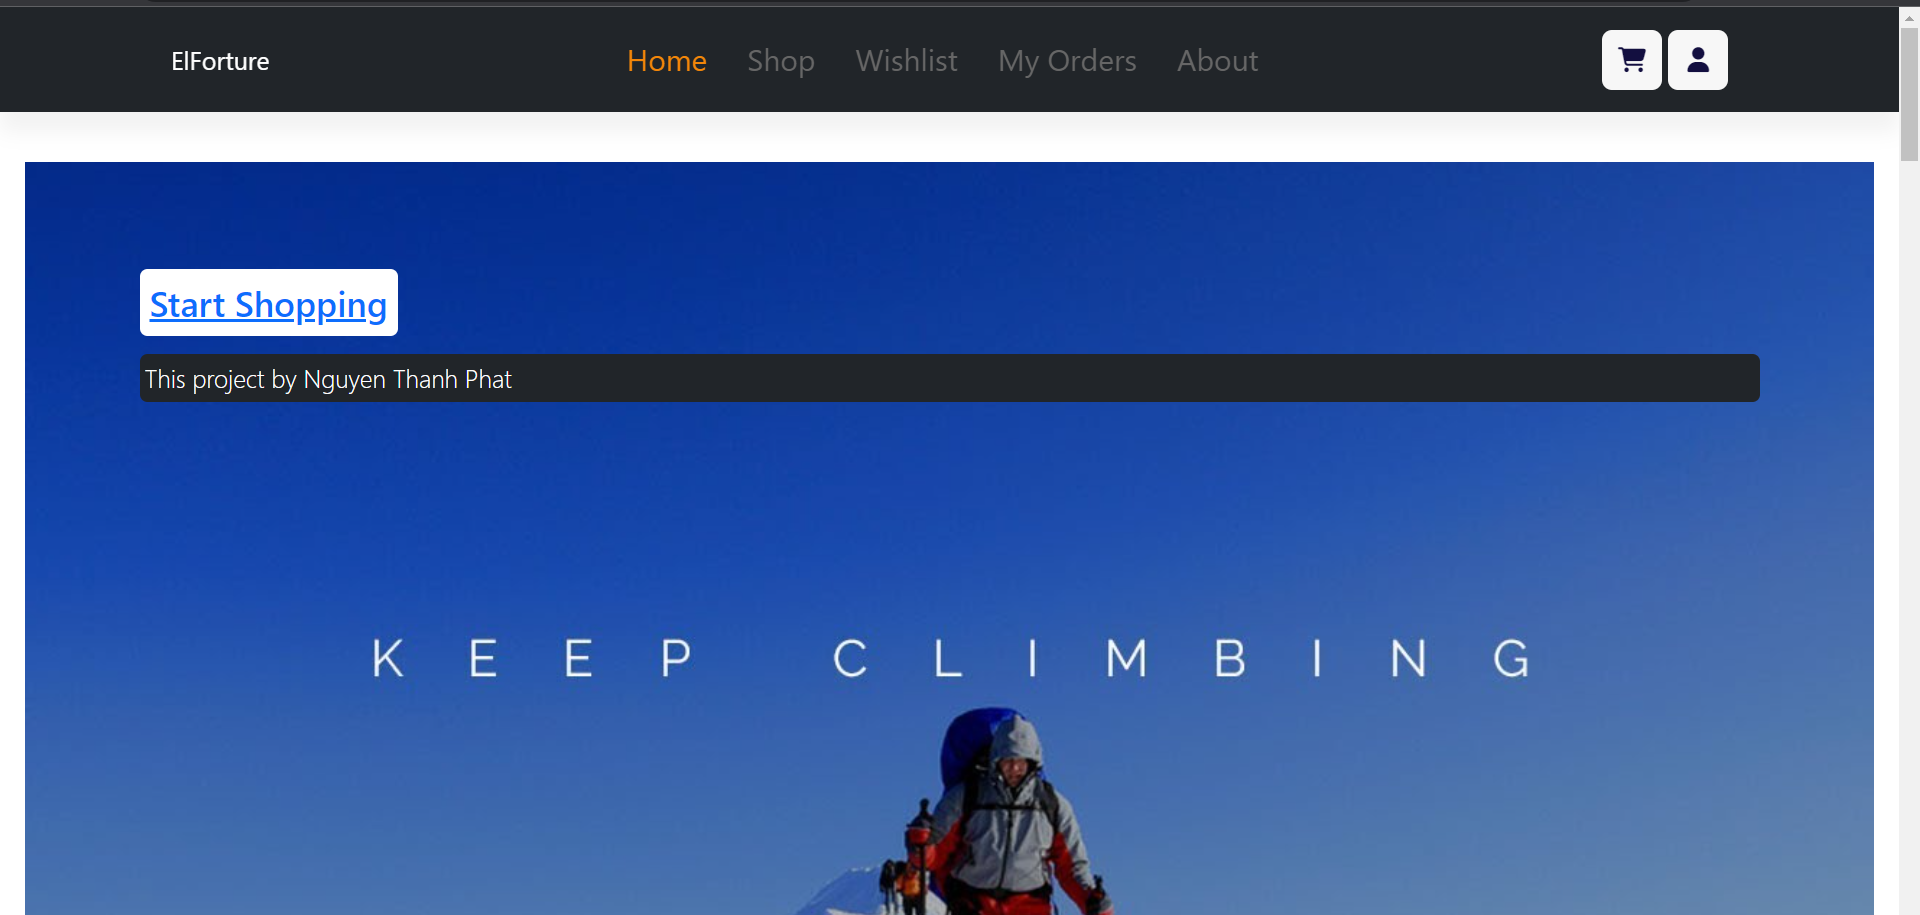
\includegraphics[width=\linewidth]{HomeView.png}
    \caption{Home View}
    \label{fig:HomeView}
\end{figure}

The HomeView allows users to easily navigate between different sections of the website. It is located at the top of the website and includes router links to the Home, Shop, Wishlist, My Orders, and Cart pages.

Additionally, it provides a user account icon for logged-in users, displaying a dropdown menu with options to access login and register, the Admin page or sign out. The menu bar also includes a hamburger icon that toggles the visibility of the main navigation links when the screen size is small.
\subsection{Authentication}
User Authentication function is a crucial part of the E-Commerce application. It allows users to create a new account or log into an existing one. This function is essential for personalizing the user experience and securing user data.

\subsubsection{Register view}
\begin{figure}[H]
    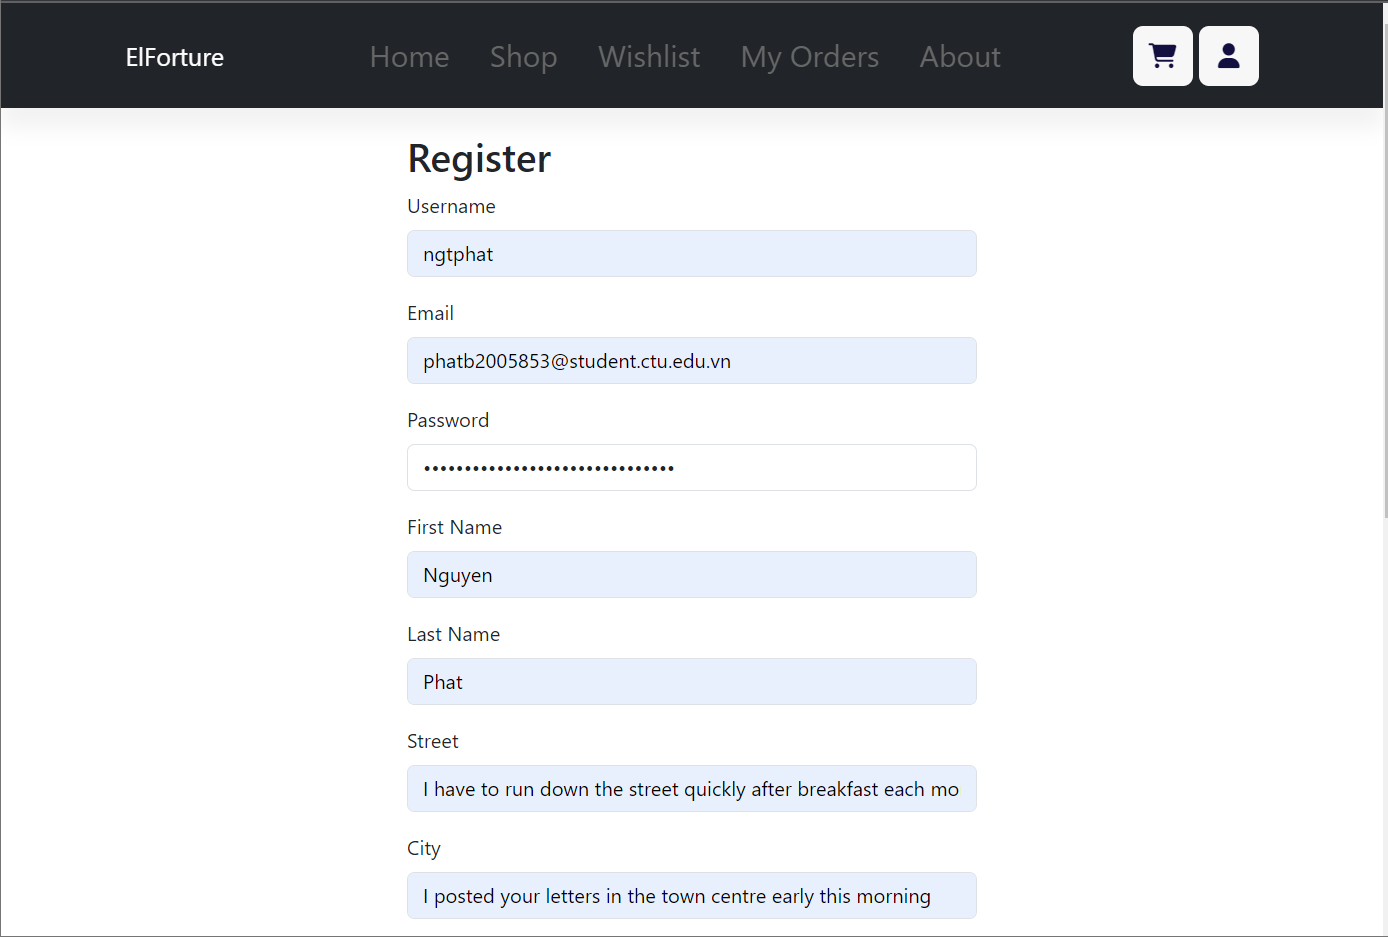
\includegraphics[width=\linewidth]{RegisterView.png}
    \caption{Register view}
    \label{fig:RegisterView}
\end{figure}

The Register feature enables new users to create an account by providing necessary details such as their name, email, and password. Once the account is created, users can access all features of the E-Commerce application.

\subsubsection{Login view}
\begin{figure}[H]
    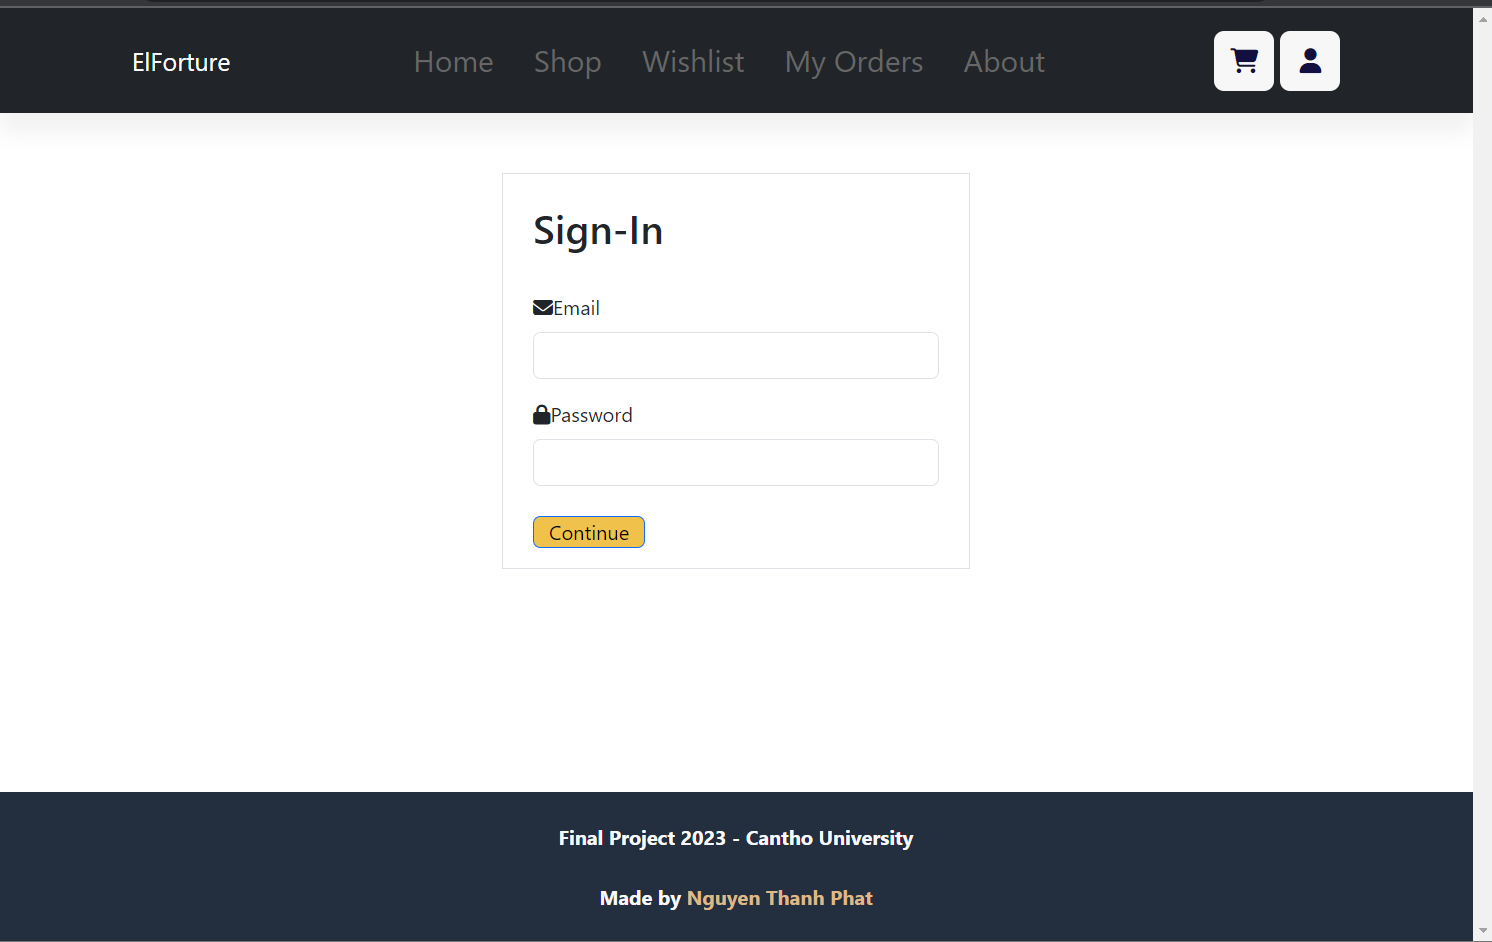
\includegraphics[width=\linewidth]{LoginView.png}
    \caption{Login view}
    \label{fig:LoginView}
\end{figure}

The Login feature allows returning users to access their accounts by entering their registered email and password. Upon successful login, users are redirected to the home page and can navigate through the application as authenticated users.

\subsection{Product browse}
\subsubsection{Search by filter (Shopping browse)}
\begin{figure}[H]
    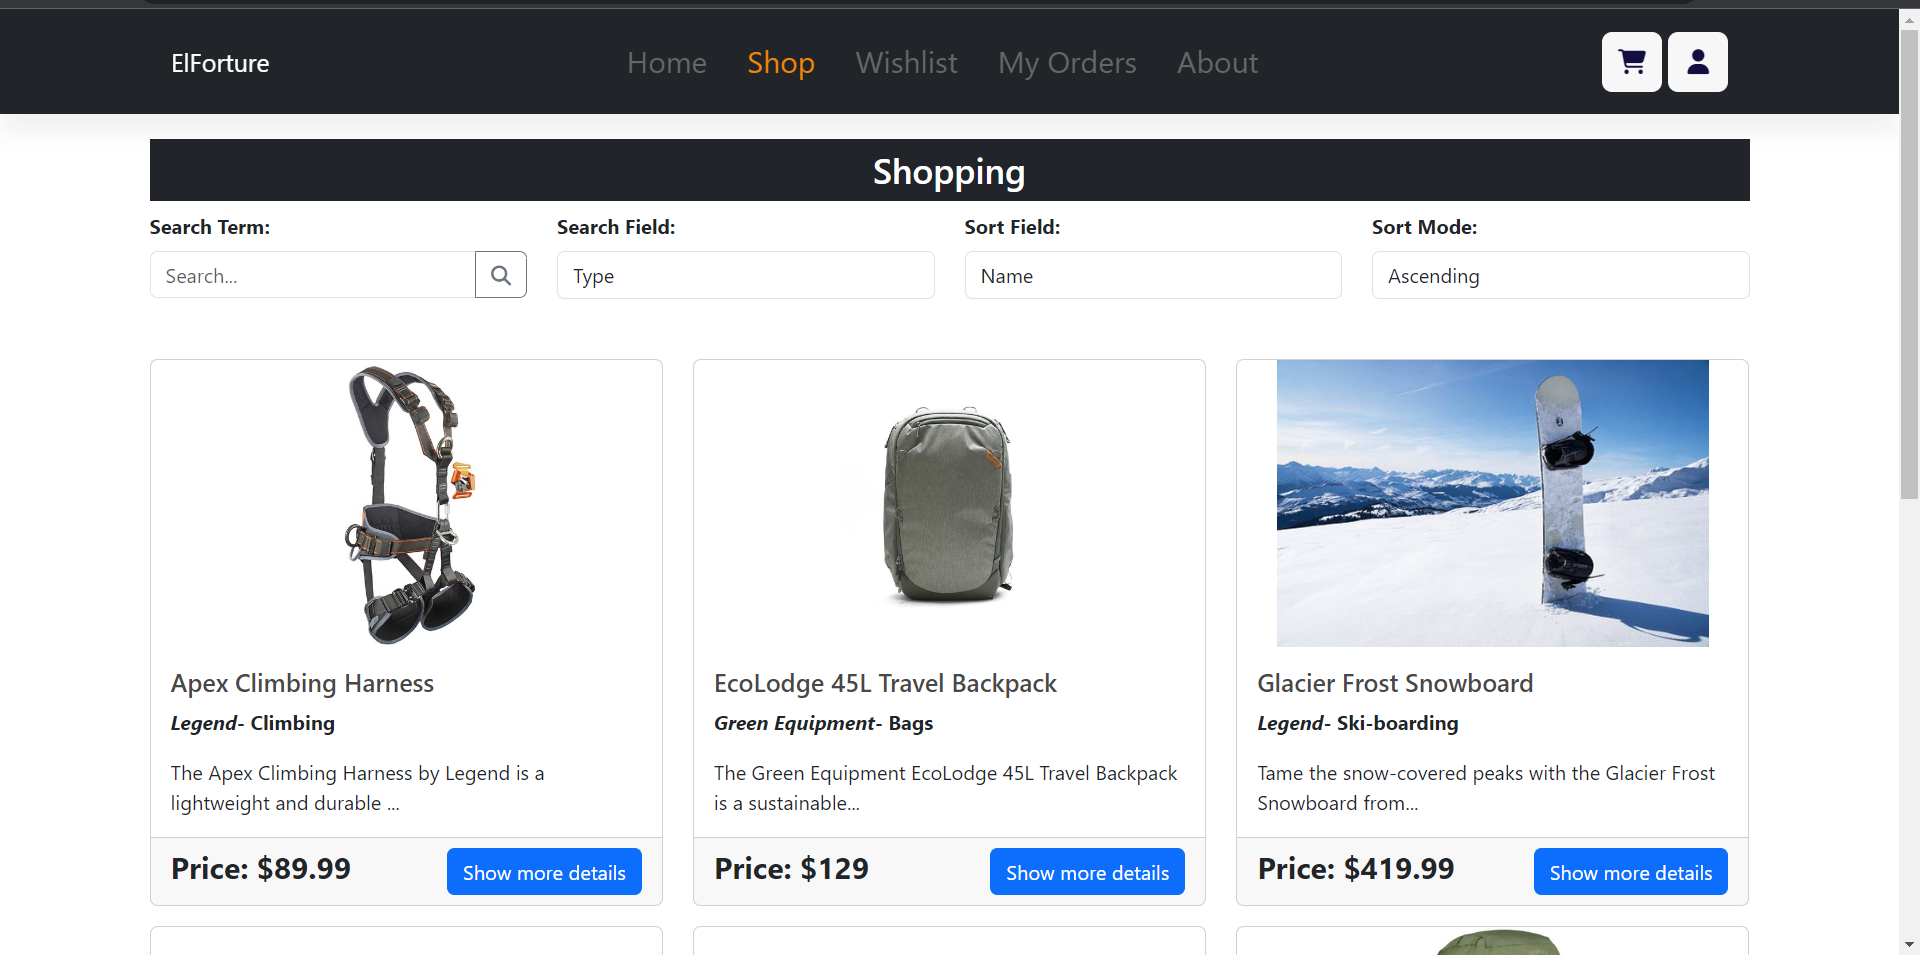
\includegraphics[width=\linewidth]{ShoppingView.png}
    \caption{Shopping View}
    \label{fig:ShoppingView}
\end{figure}
The Product Search function is an essential part of the E-Commerce application. It allows users to search for products available on the platform. This function includes several components: View All Products, Search Products By Query, Filter Products By Type, and Sort Products.

\subsubsection{Product Details Page}
\begin{figure}[H]
    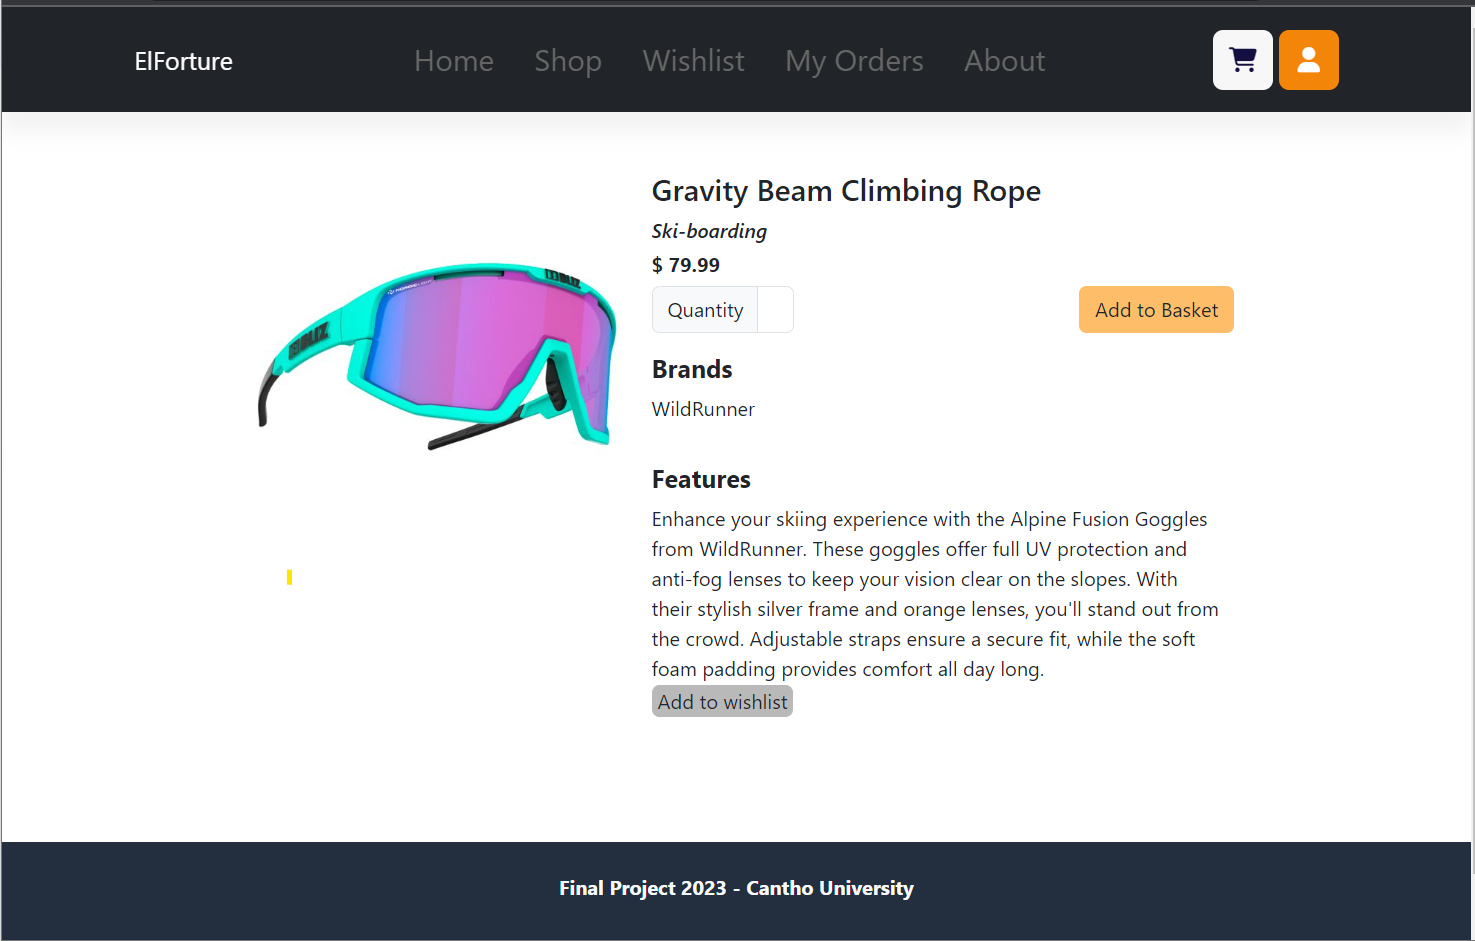
\includegraphics[width=\linewidth]{ProductDetailView.png}
    \caption{Product Detail View}
    \label{fig:ProductDetailView}
\end{figure}
The Product Search function is an essential part of the E-Commerce application. It allows users to search for products available on the platform. This function includes several components: View All Products, Search Products By Query, Filter Products By Type, and Sort Products.
Add to Cart and Add to Wishlist notification.

\subsection{Wishlist}
\begin{figure}[H]
    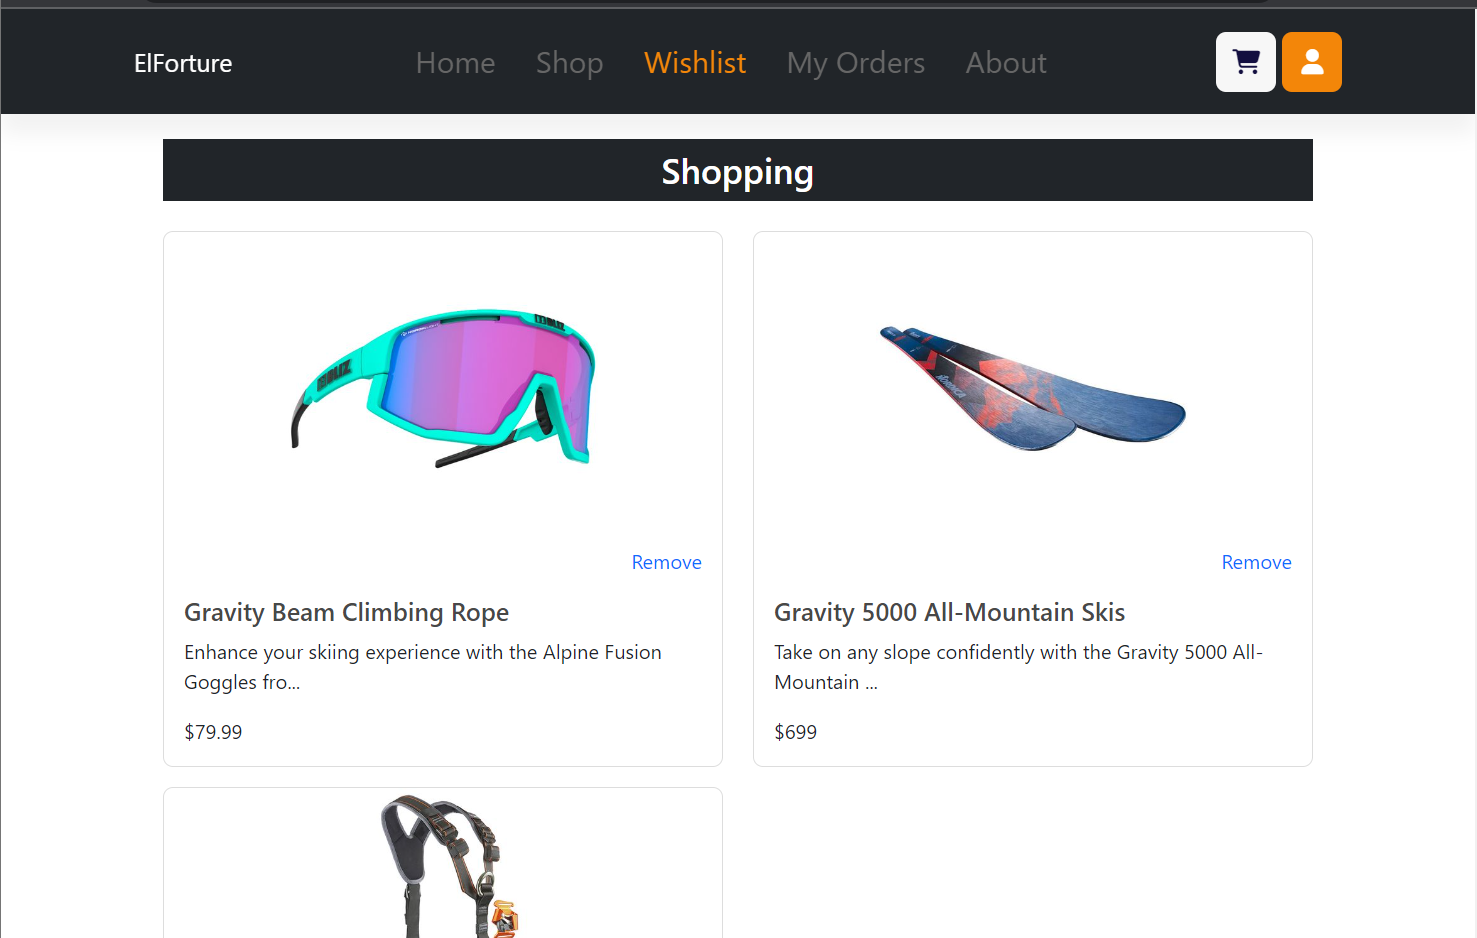
\includegraphics[width=\linewidth]{WishlistView.png}
    \caption{Wishlist vieww}
    \label{fig:WishlistView}
\end{figure}
The Wishlist page displays a list of products that the user has added to their wishlist. It allows users to view and manage their wishlist items, including adding them to the cart or removing them. Each wishlist item includes a product image, name , overall description, price and option to access more details about the product.


\subsection{BasketView}
\begin{figure}[H]
    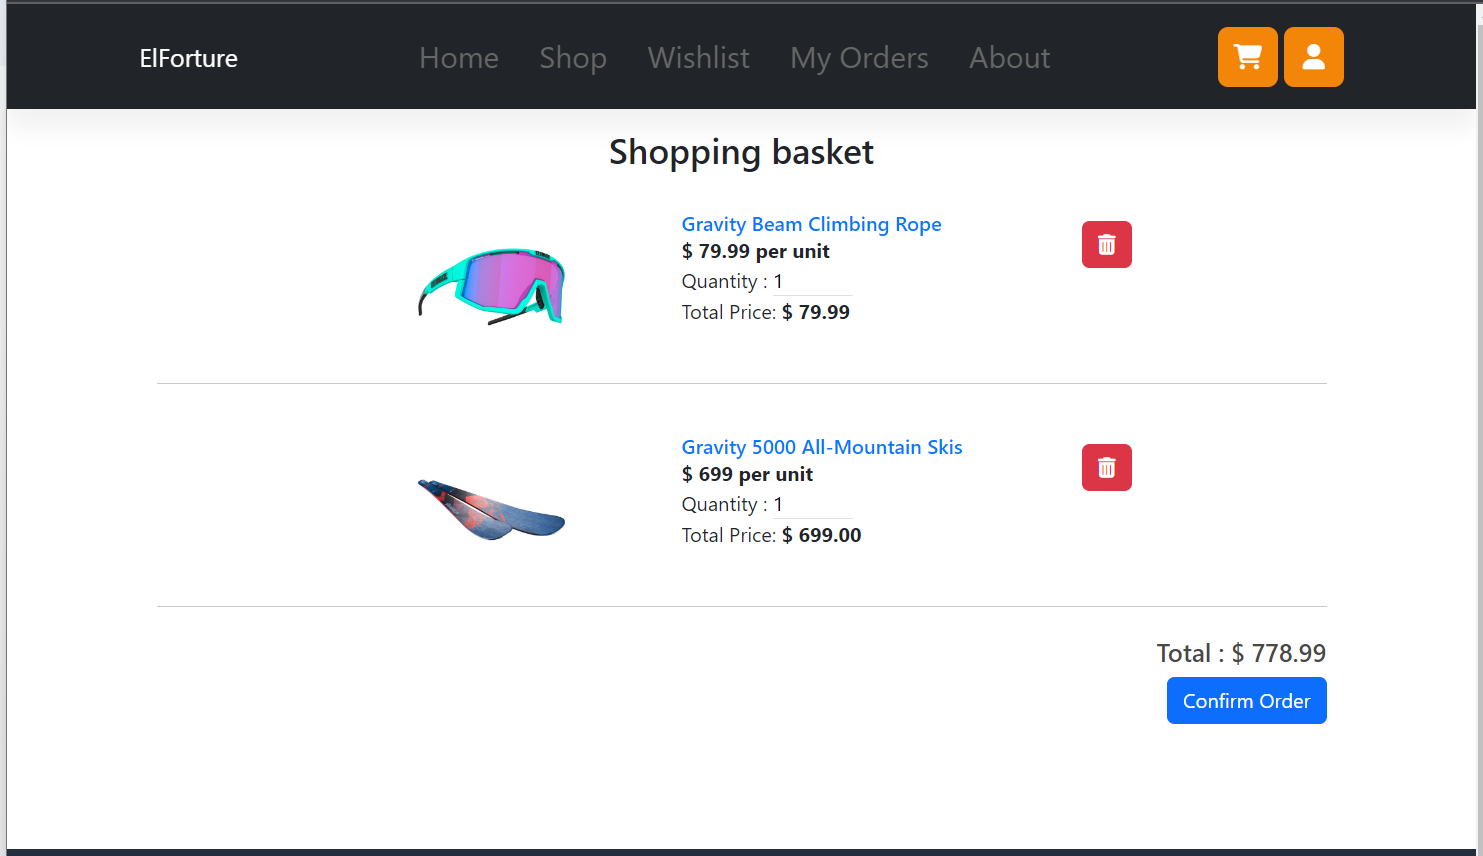
\includegraphics[width=\linewidth]{BasketView.png}
    \caption{Basket View}
    \label{fig:BasketView}
\end{figure}

The BasketView displays a list of products in the user's shopping cart, allowing them to view, update quantities, and remove items. Users can proceed to checkout to complete the purchase.

Process Payment: This page is calling and waiting for a redirect website  from Stripe Payment Gateway which processes in  Server-side API.

\subsubsection{ToCheckOutView}

\begin{figure}[H]
    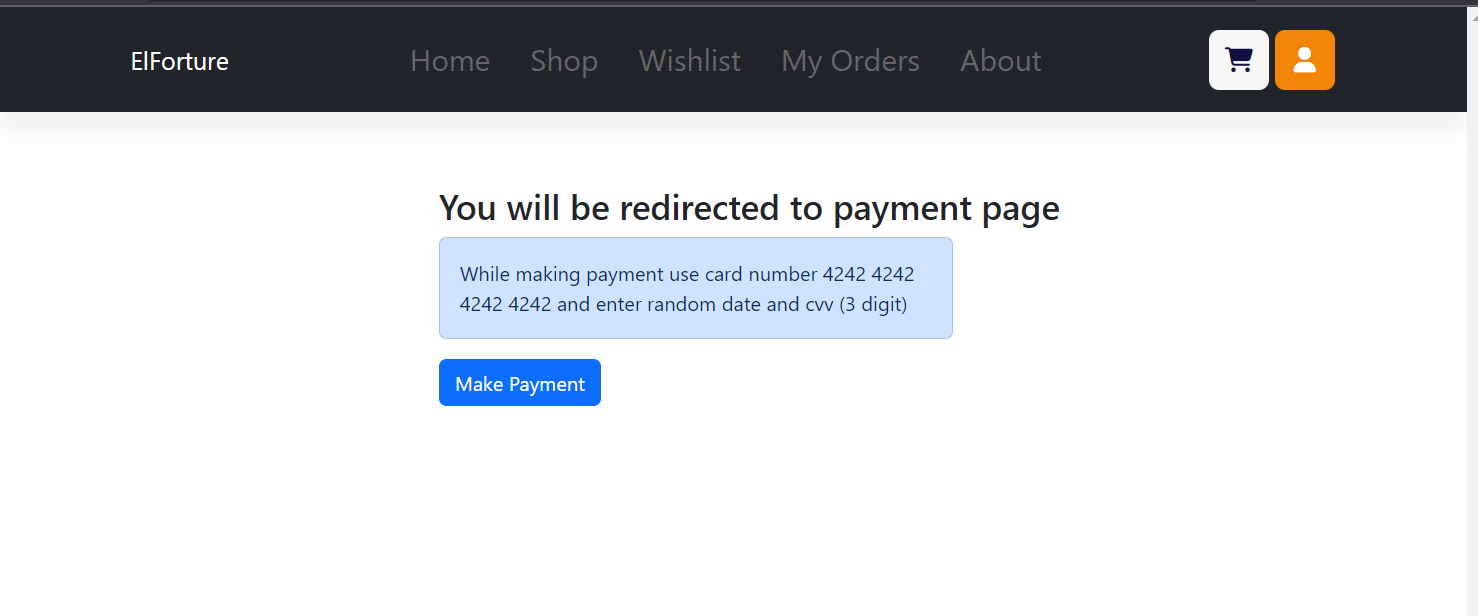
\includegraphics[width=\linewidth]{ProcedToPaymentView.png}
    \caption{Proced To Payment View}
    \label{fig:ProcedToPaymentView}
\end{figure}

Then user will direct to Payment page of  Stripe:
\begin{figure}[H]
    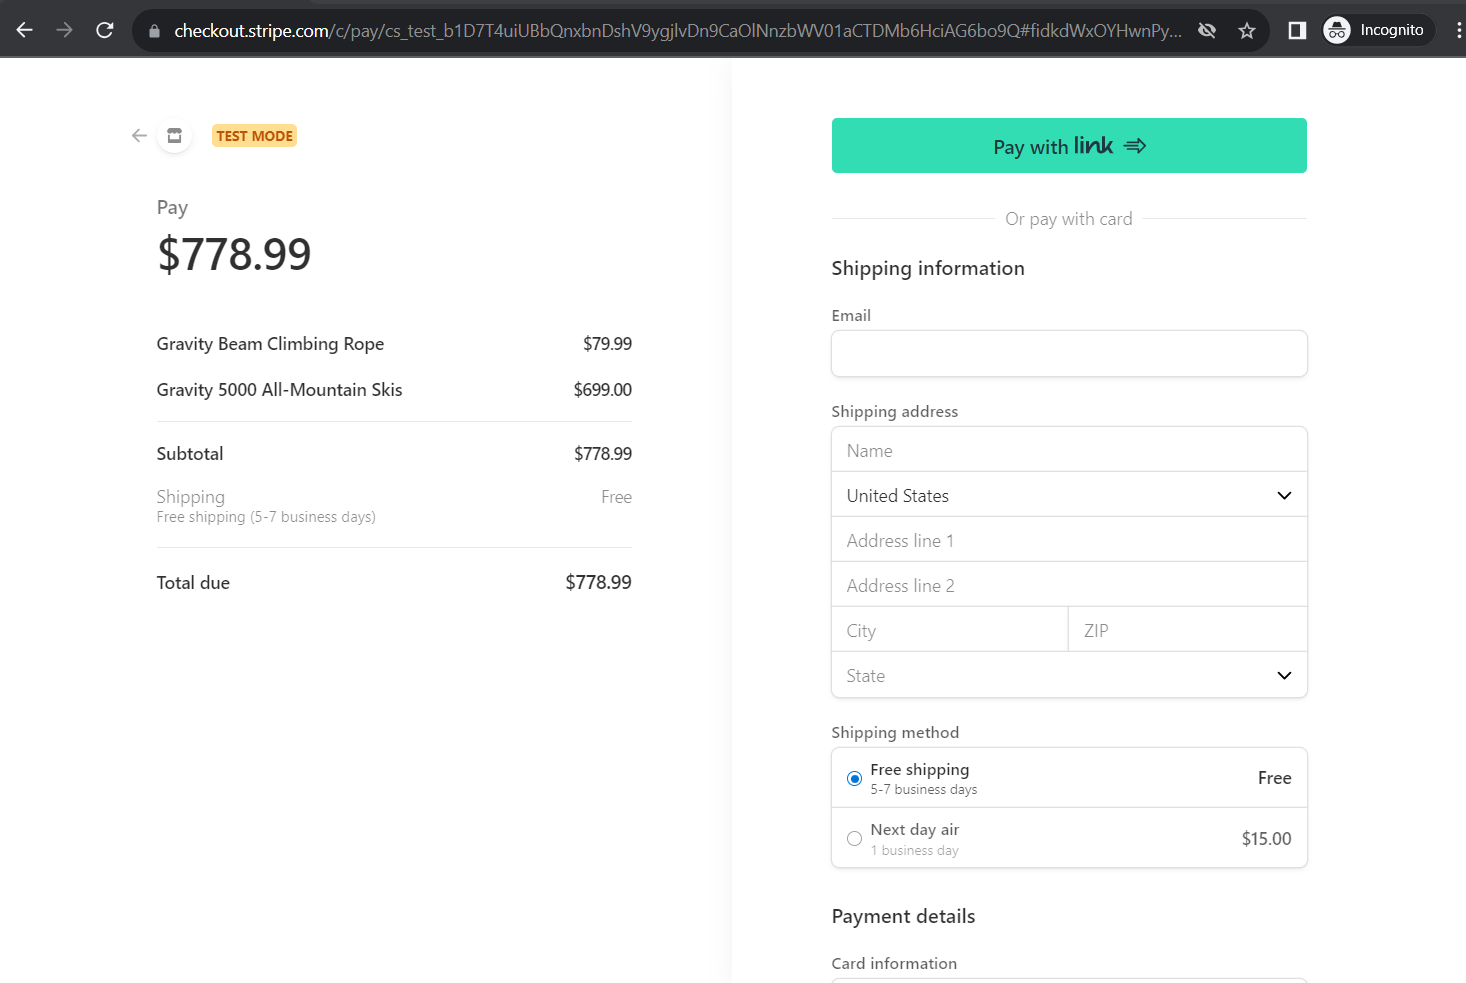
\includegraphics[width=\linewidth]{STRIPECheckoutPayment.png}
    \caption{Payment page of  Stripe}
    \label{fig:STRIPECheckoutPayment}
\end{figure}

\begin{figure}[H]
    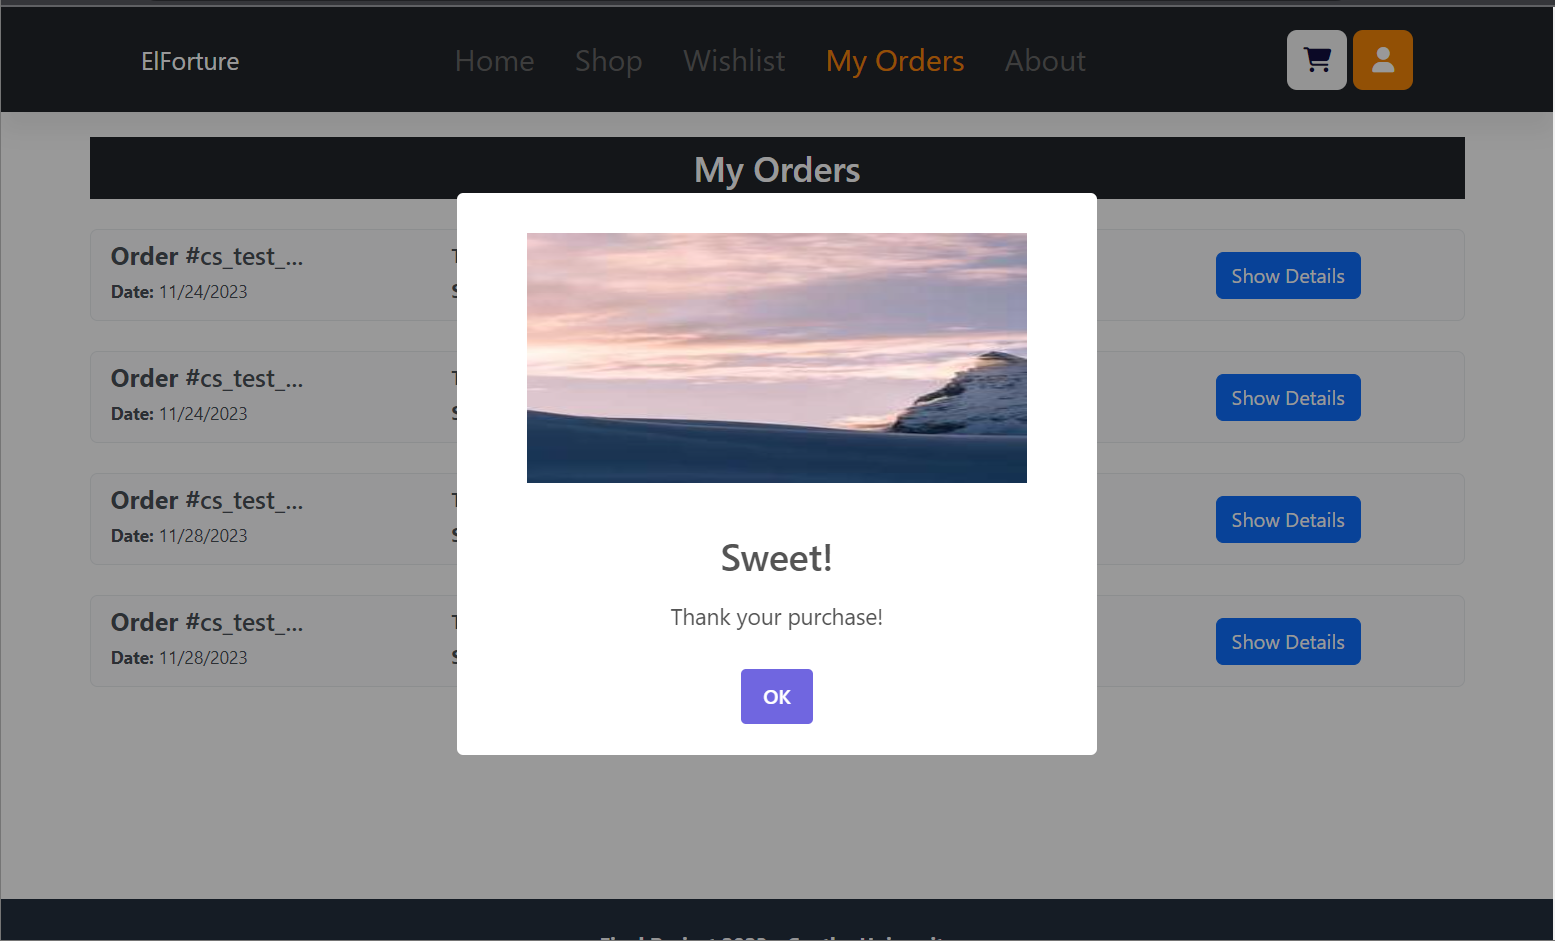
\includegraphics[width=\linewidth]{SucessOrder.png}
    \caption{Order successfully}
    \label{fig:SucessOrder}
\end{figure}

\subsection{Admin - Catalog Type}
The Administrator - Type Management function is a crucial part of the E-Commerce application. It allows the administrator to manage the product types available on the platform. This function includes several components: View All Categories, View Type By ID, Create Type, and Update Type.
\subsubsection[]{View All Categories}
The View All Categories component retrieves all the types from the database.
\begin{figure}[H]
    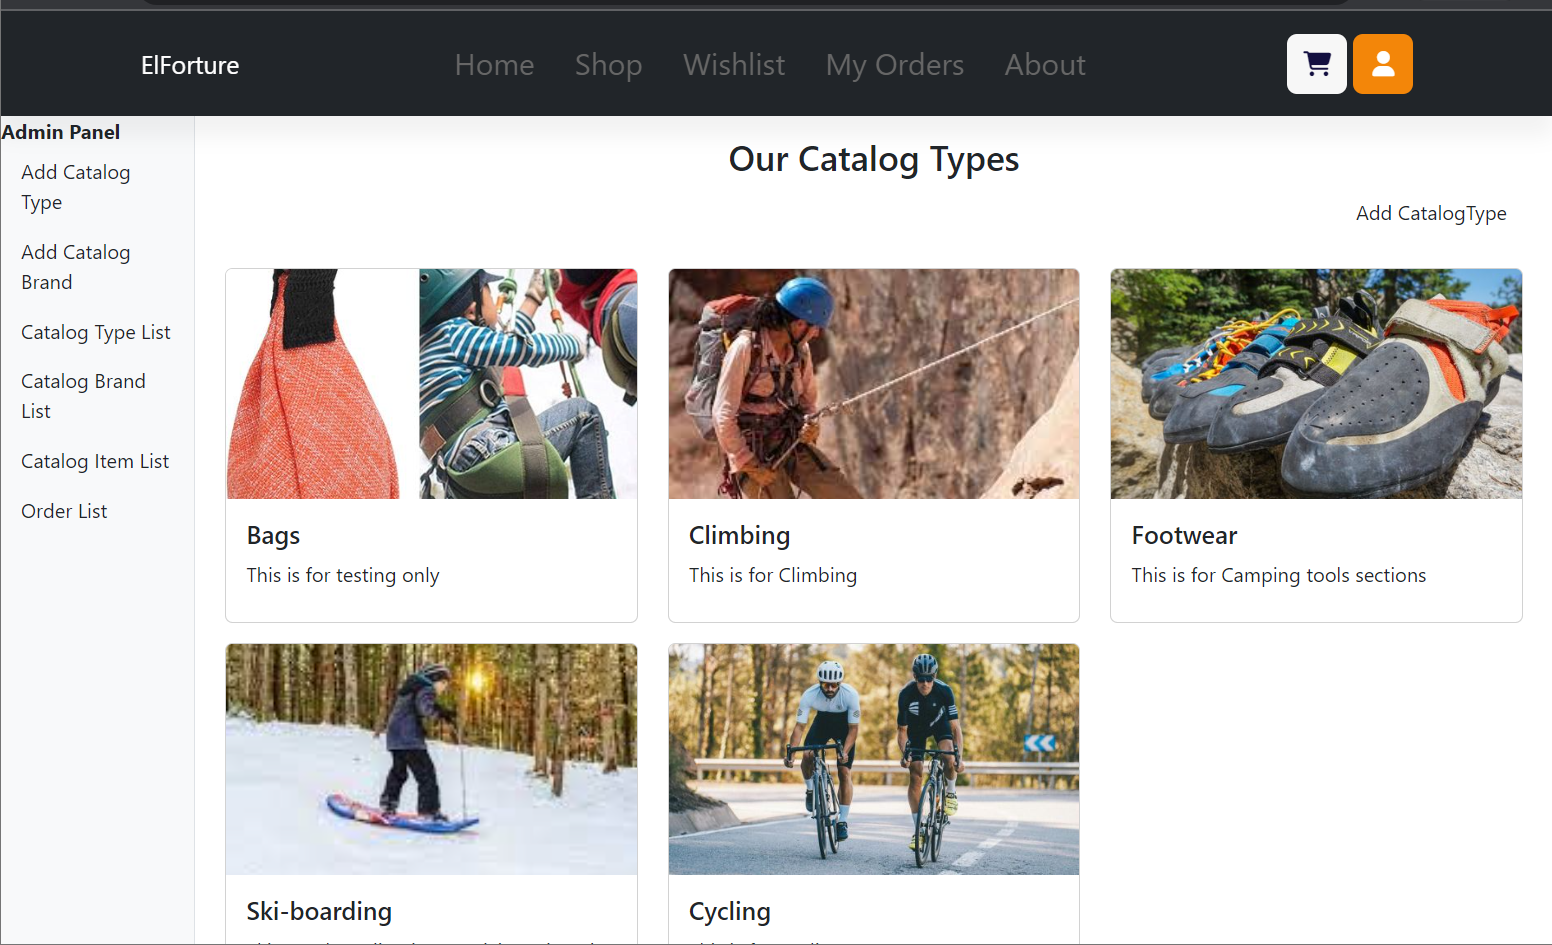
\includegraphics[width=\linewidth]{TypeList.png}
    \caption{View Types}
    \label{fig:TypeList}
\end{figure}

\subsubsection[]{Add new type}
TThe Add Category component allows the administrator to add a new type to the database.
\begin{figure}[H]
    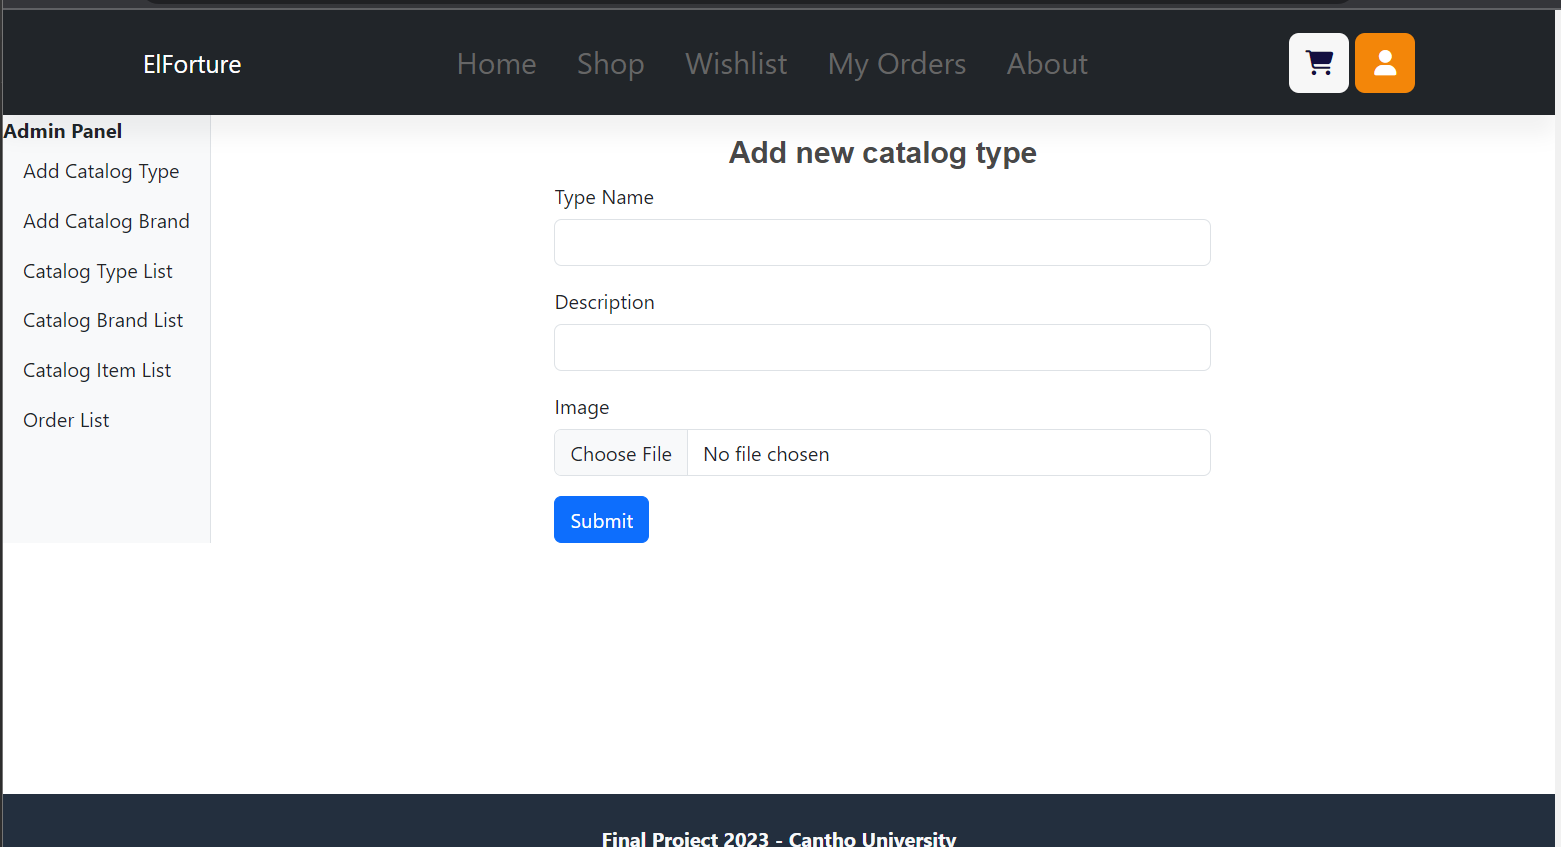
\includegraphics[width=\linewidth]{AdddNewCateglory.png}
    \caption{View Types}
    \label{fig:AdddNewCateglory}
\end{figure}

\subsection{Admin - Catalog Brand}
The Administrator - Brand Management function is a crucial part of the E-Commerce application. It allows the administrator to manage the product types available on the platform. This function includes several components: View All Brands, View Brand By ID, Create Brand, and Update Brand.
\subsubsection[]{View All Brands}
The View All Categories component retrieves all the brands from the database.
\begin{figure}[H]
    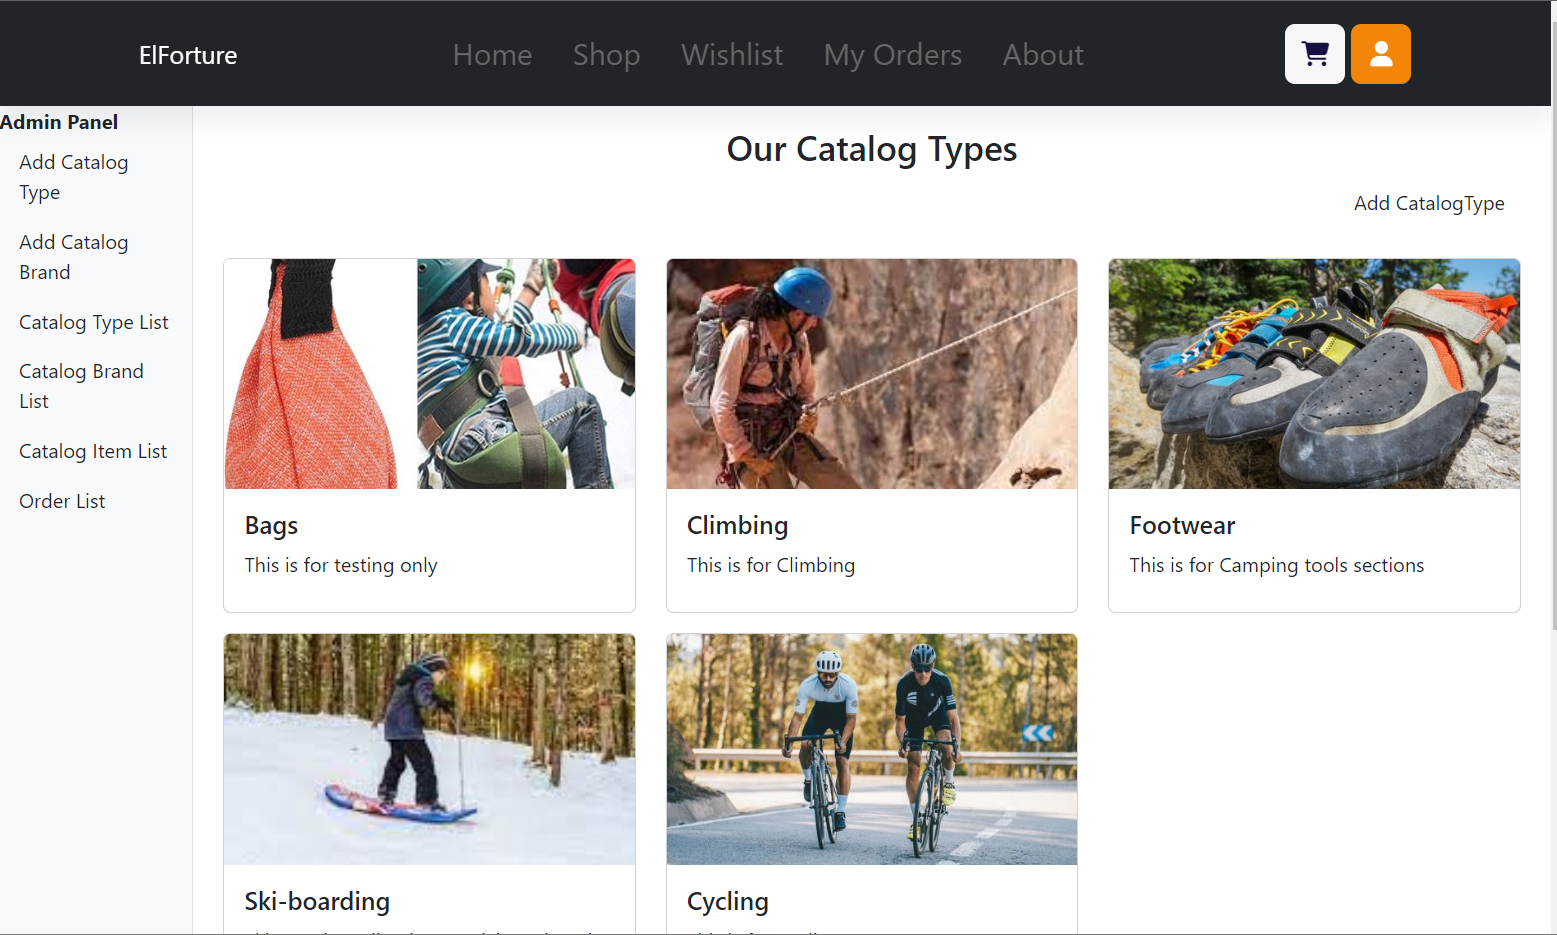
\includegraphics[width=\linewidth]{BrandView.png}
    \caption{Brand View Types}
    \label{fig:BrandView}
\end{figure}

\subsubsection[]{Add new brand}
TThe Add Brand component allows the administrator to add a new type to the database.
\begin{figure}[H]
    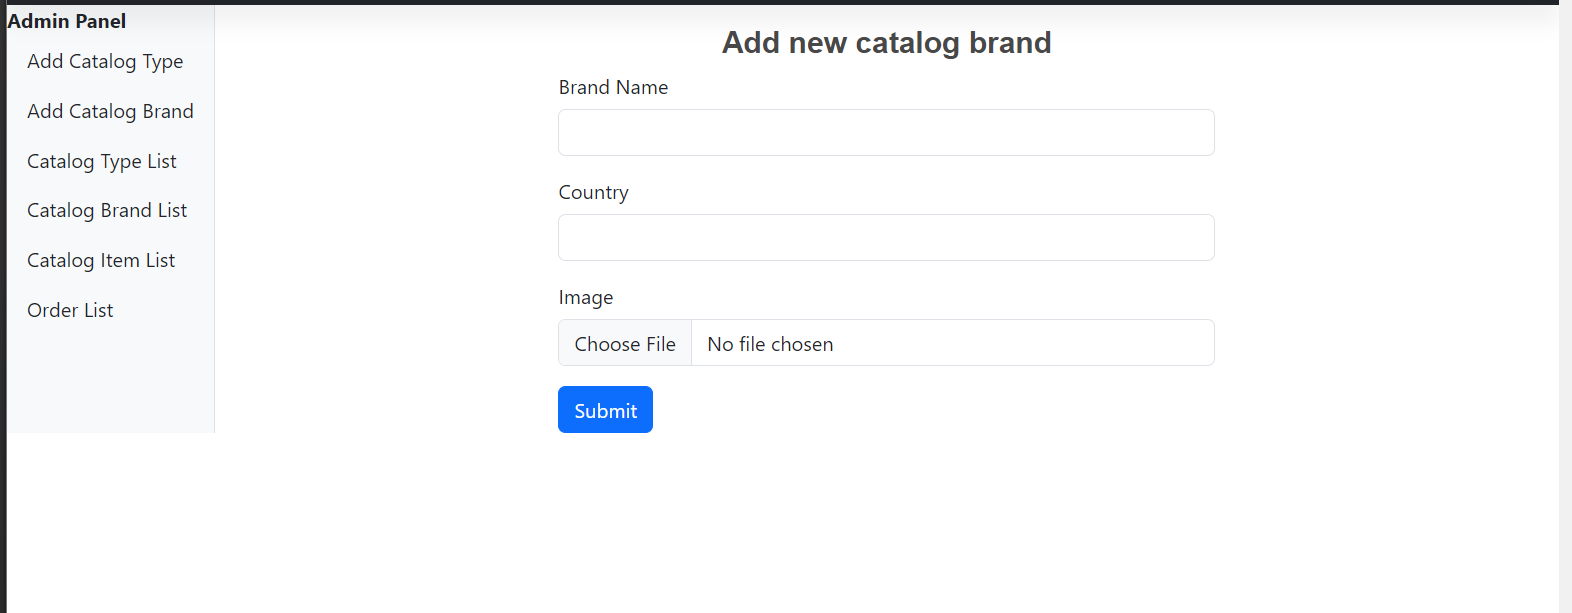
\includegraphics[width=\linewidth]{AdddNewBrand.png}
    \caption{Addd New Brand}
    \label{fig:AdddNewBrand}
\end{figure}

\subsection{Admin - Catalog Product}
The Administrator - Product Management function is a key part of the E-Commerce application. It allows the administrator to manage the products available on the platform. This function includes several components: Get All Products, Get Product By ID, Add Product, Update Product Information.
\subsubsection[]{View All Products}
The View All Categories component retrieves all the brands from the database.
\begin{figure}[H]
    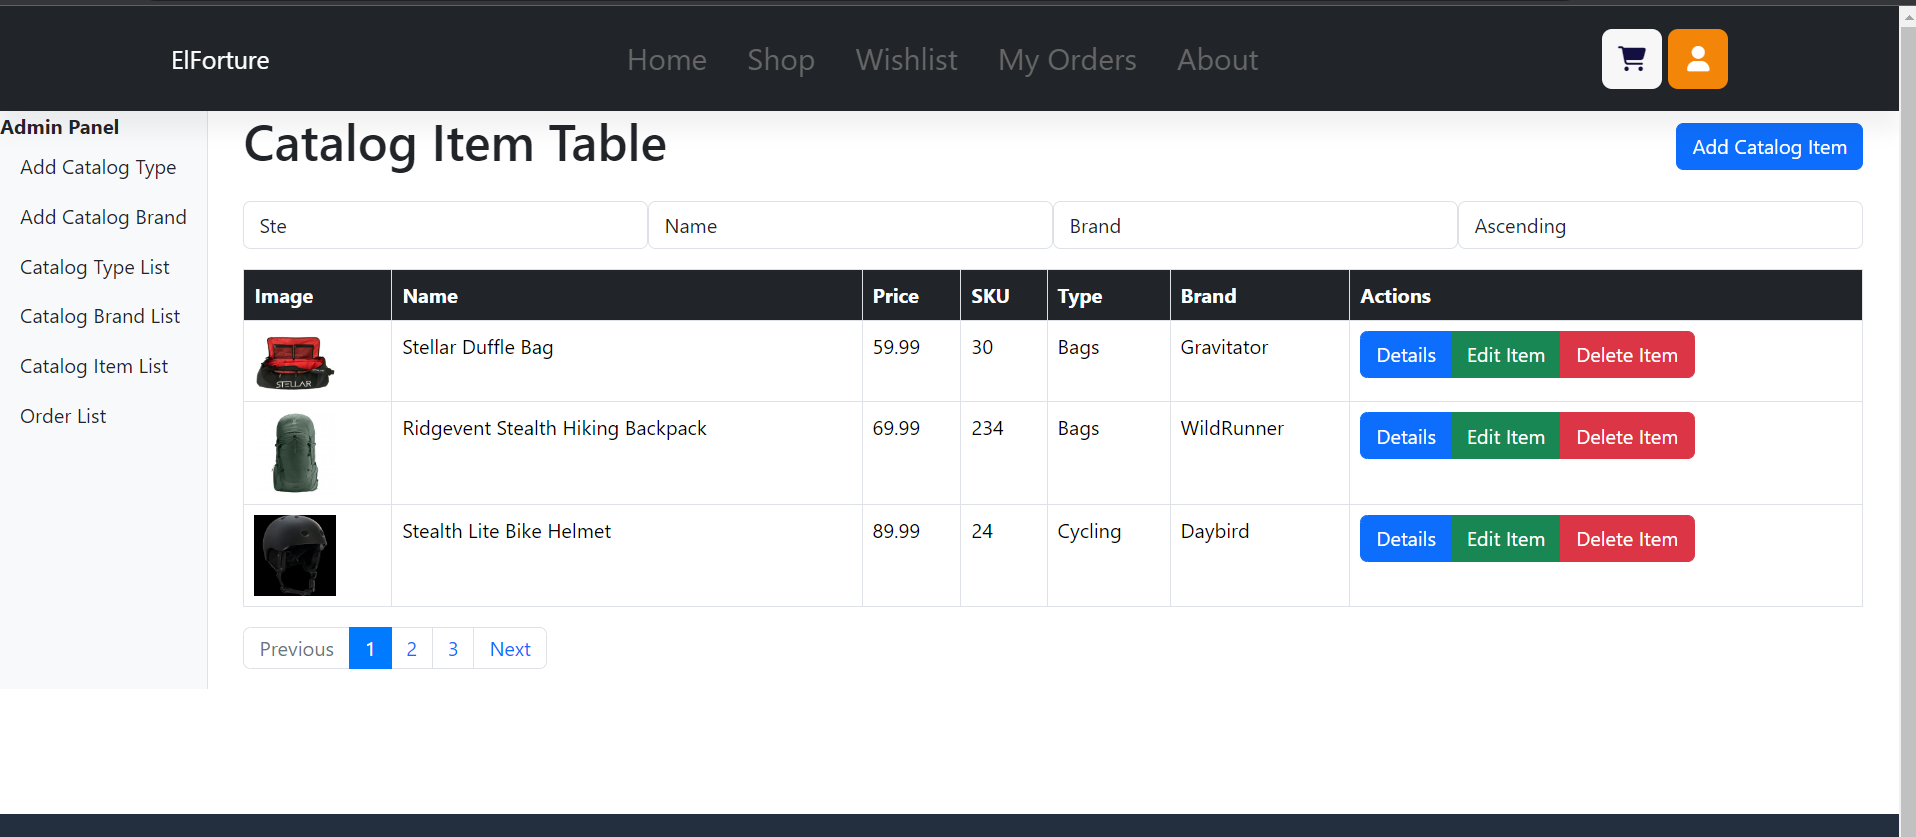
\includegraphics[width=\linewidth]{adminProductView.png}
    \caption{View Types}
    \label{fig:adminProductView}
\end{figure}

\subsubsection[]{Add new product}
TThe Add Category component allows the administrator to add a new product to the database.
\begin{figure}[H]
    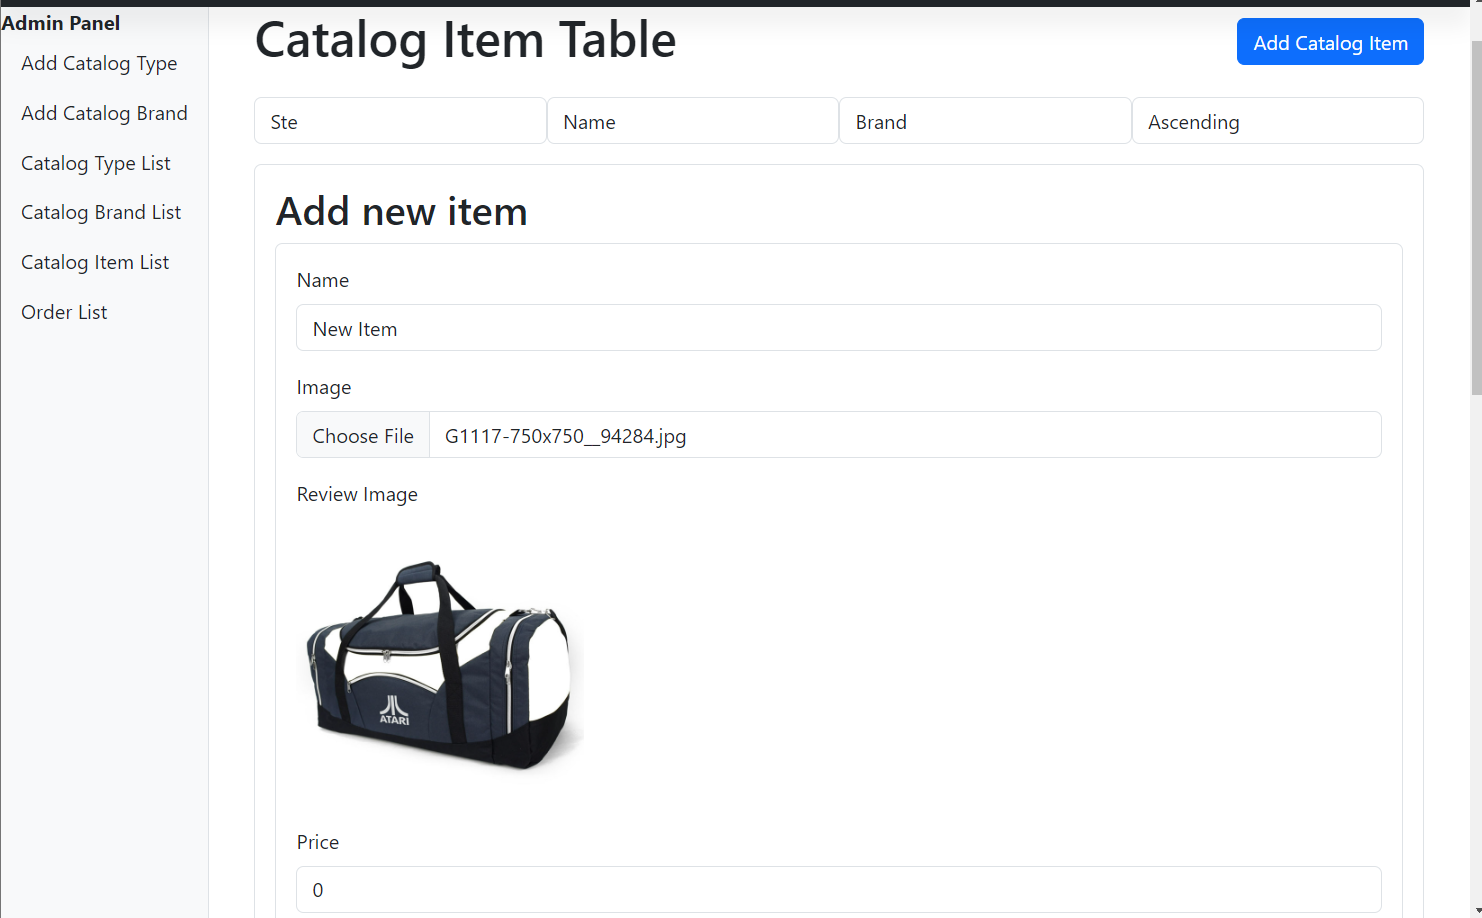
\includegraphics[width=\linewidth]{AddnNewProduct.png}
    \caption{add Catlog Item}
    \label{fig:AddnNewProduct}
\end{figure}

\subsubsection[]{Edit}
TThe Add Category component allows the administrator to add a new product to the database.
\begin{figure}[H]
    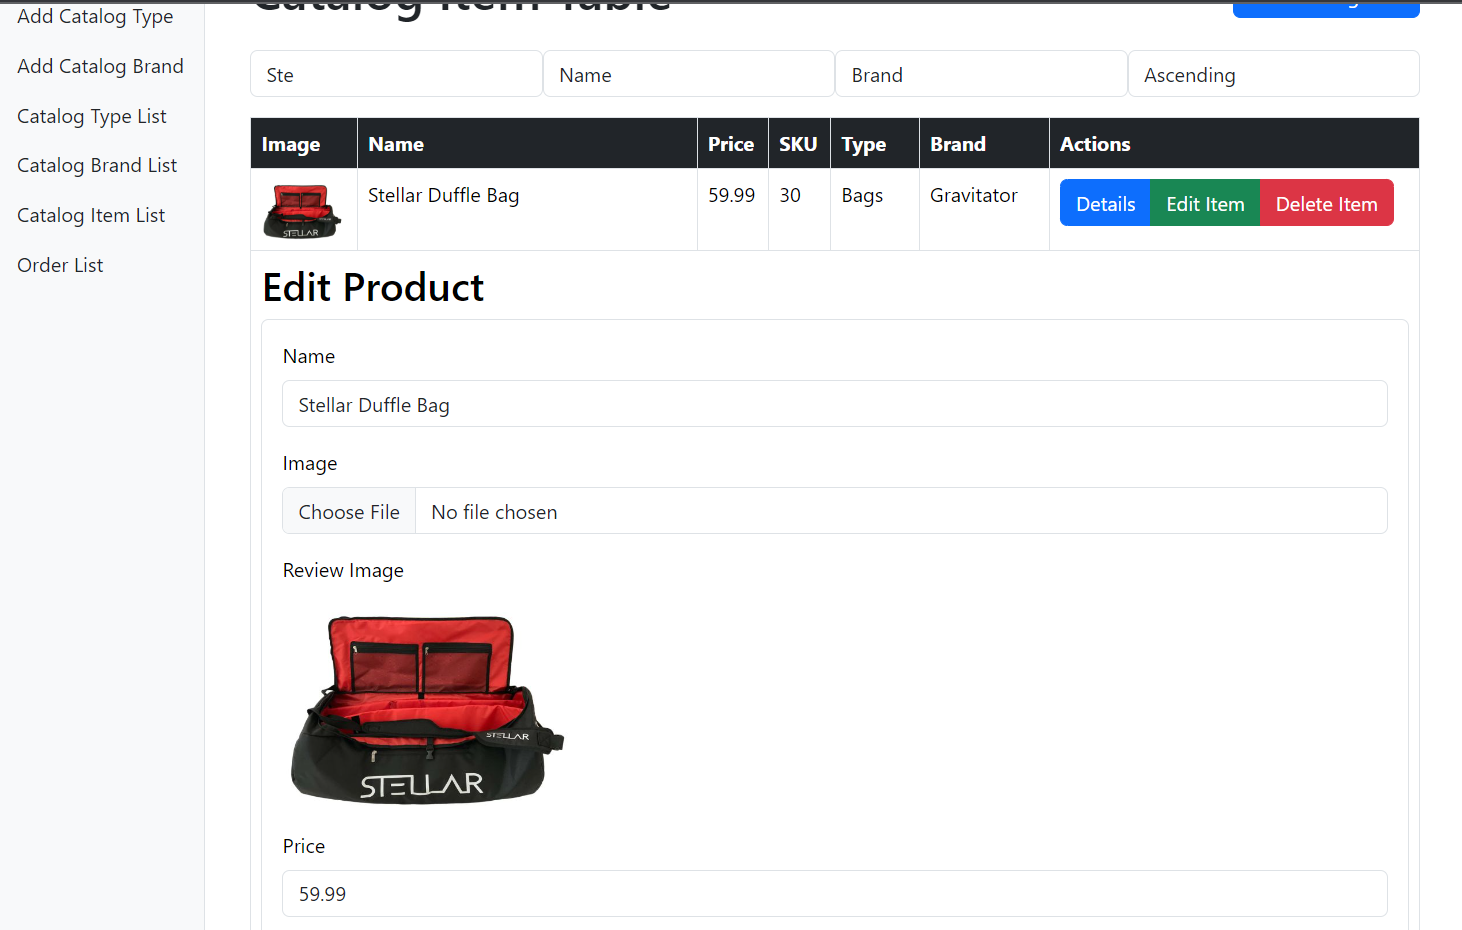
\includegraphics[width=\linewidth]{editCatlogItem.png}
    \caption{edit Catlog Item}
    \label{fig:editCatlogItem}
\end{figure}

\subsection{Admin - Customer Orders}
The Administrator - Order Management function is a vital part of the E-Commerce application. It allows the administrator to manage the orders placed on the platform. This function includes several components: View All Orders, View Order By ID, and Update Order Status.
\subsubsection[]{View All Orders}
The View All Categories component retrieves all the brands from the database.
\begin{figure}[H]
    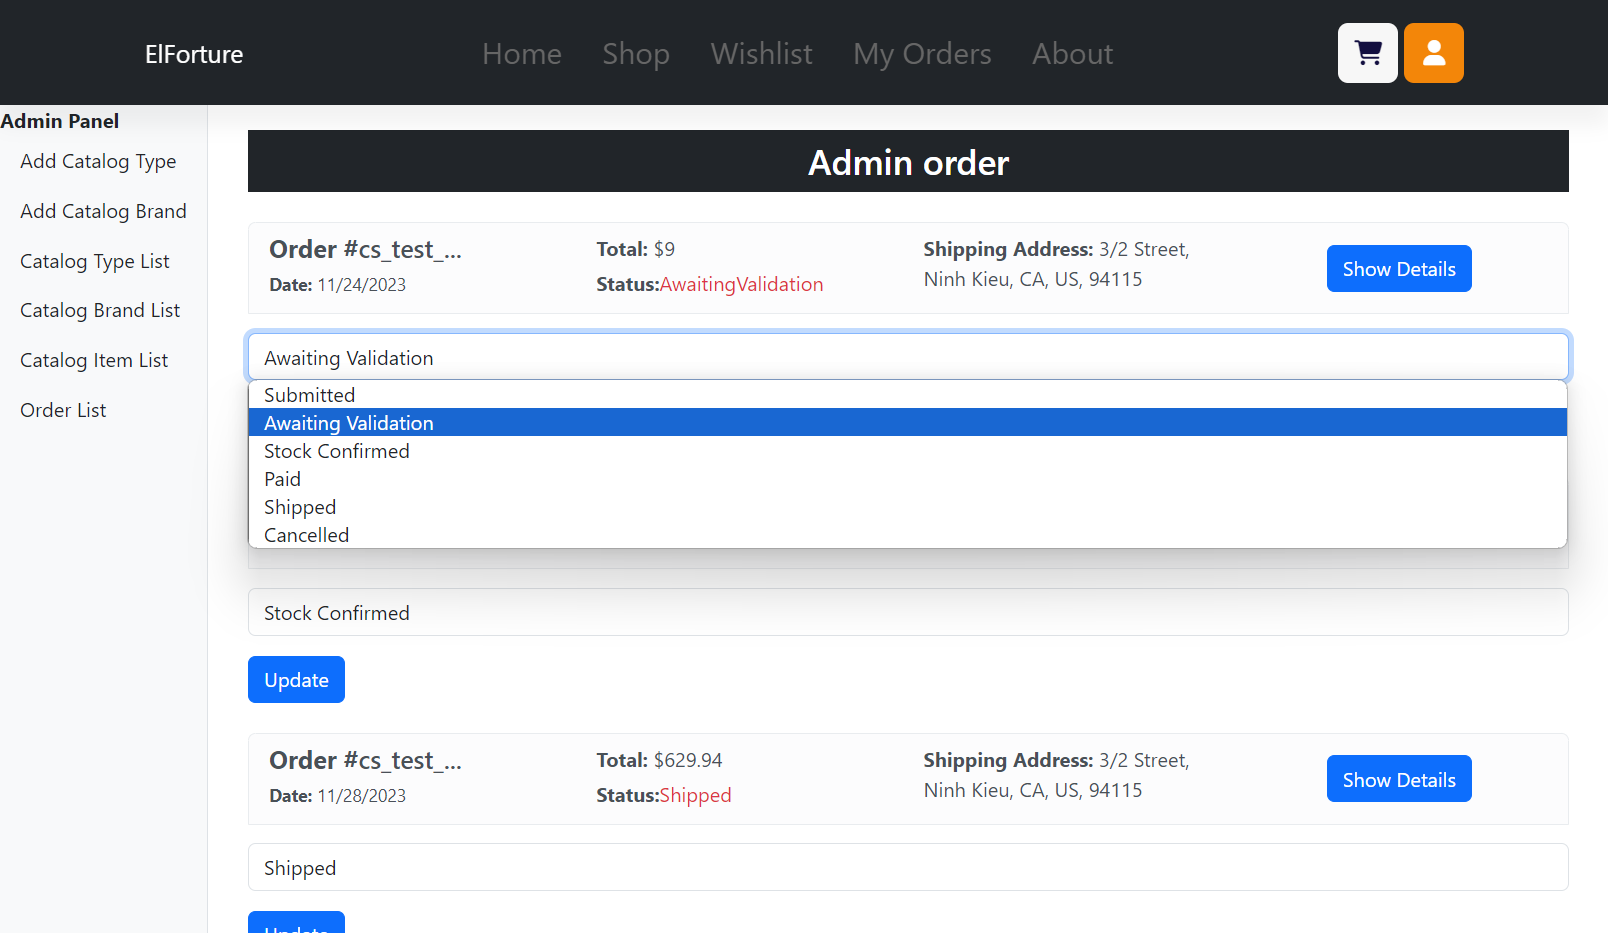
\includegraphics[width=\linewidth]{AdminOrderListView.png}
    \caption{View All Orders}
    \label{fig:AdminOrderListView}
\end{figure}